\refstepcounter{section}
\section*{Lecture 11: Finding Geodesics}
\addcontentsline{toc}{section}{Lecture 11: Finding Geodesics}
Since a particle following the geodesics have no \textit{proper acceleration} in a local inertial frame, the geodesics generally represent the `straightest' path between two points in a space. Let us take the example for the shortest distance between two cities $A$ and $B$ on the Earth. Since the Earth can be assumed to be a sphere, we just need to find the geodesic equation on $\mathbb{S}^2$ and then solve it.
\begin{figure}[H]
    \centering 
    

\tikzset{every picture/.style={line width=0.75pt}} %set default line width to 0.75pt        

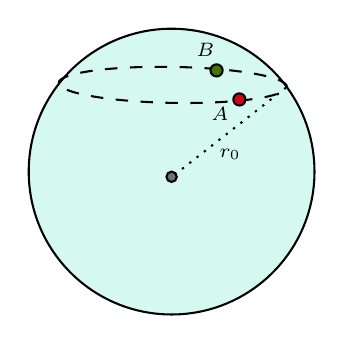
\begin{tikzpicture}[x=0.75pt,y=0.75pt,yscale=-1,xscale=1]
%uncomment if require: \path (0,300); %set diagram left start at 0, and has height of 300

%Shape: Circle [id:dp9662332410710763] 
\draw  [fill={rgb, 255:red, 80; green, 227; blue, 194 }  ,fill opacity=0.24 ] (220.57,135.84) .. controls (220.57,97.82) and (251.39,67) .. (289.41,67) .. controls (327.43,67) and (358.25,97.82) .. (358.25,135.84) .. controls (358.25,173.86) and (327.43,204.68) .. (289.41,204.68) .. controls (251.39,204.68) and (220.57,173.86) .. (220.57,135.84) -- cycle ;
%Shape: Ellipse [id:dp33389267024299074] 
\draw  [dash pattern={on 4.5pt off 4.5pt}] (235,93.11) .. controls (235.09,88.32) and (259.77,84.87) .. (290.14,85.4) .. controls (320.5,85.93) and (345.05,90.24) .. (344.97,95.03) .. controls (344.88,99.82) and (320.2,103.27) .. (289.83,102.74) .. controls (259.47,102.21) and (234.92,97.9) .. (235,93.11) -- cycle ;
%Shape: Circle [id:dp651906164523799] 
\draw  [fill={rgb, 255:red, 208; green, 2; blue, 27 }  ,fill opacity=1 ] (319.15,101.07) .. controls (319.15,102.69) and (320.46,104) .. (322.07,104) .. controls (323.69,104) and (325,102.69) .. (325,101.07) .. controls (325,99.46) and (323.69,98.15) .. (322.07,98.15) .. controls (320.46,98.15) and (319.15,99.46) .. (319.15,101.07) -- cycle ;
%Shape: Circle [id:dp3587972313578581] 
\draw  [fill={rgb, 255:red, 65; green, 117; blue, 5 }  ,fill opacity=1 ] (308.15,87.07) .. controls (308.15,88.69) and (309.46,90) .. (311.07,90) .. controls (312.69,90) and (314,88.69) .. (314,87.07) .. controls (314,85.46) and (312.69,84.15) .. (311.07,84.15) .. controls (309.46,84.15) and (308.15,85.46) .. (308.15,87.07) -- cycle ;
%Shape: Circle [id:dp4357923860514987] 
\draw  [fill={rgb, 255:red, 0; green, 0; blue, 0 }  ,fill opacity=0.52 ] (286.92,138.34) .. controls (286.92,139.72) and (288.03,140.83) .. (289.41,140.83) .. controls (290.79,140.83) and (291.91,139.72) .. (291.91,138.34) .. controls (291.91,136.96) and (290.79,135.84) .. (289.41,135.84) .. controls (288.03,135.84) and (286.92,136.96) .. (286.92,138.34) -- cycle ;
%Straight Lines [id:da4093622522467487] 
\draw  [dash pattern={on 0.84pt off 2.51pt}]  (290.91,137.34) -- (344.97,95.03) ;

% Text Node
\draw (307.15,103.47) node [anchor=north west][inner sep=0.75pt]  [font=\scriptsize]  {$A$};
% Text Node
\draw (300,72.4) node [anchor=north west][inner sep=0.75pt]  [font=\scriptsize]  {$B$};
% Text Node
\draw (311,123.4) node [anchor=north west][inner sep=0.75pt]  [font=\scriptsize]  {$r_{0}$};


\end{tikzpicture}


\end{figure}
\noindent
Intuitively, out of the infinite ways of going between those cities, we think that moving along a line of latitude would be more economical. However, let us check if that is indeed so!\\[0.2cm]
For that, note that the invariant distance on the sphere $\mathbf{S}^2$ of radius $r_0$ is:
$$ds^2 = r_0^2\dd\theta^2+r_0^2\sin^2\theta\dd\phi^2$$
From this, we can easily identity the metric and inverse metric for the space as:
$$[g]\equiv \mqty(r_0^2 & 0 \\ 0 & r_0^2\sin^2\theta)\qquad \qquad [g^{-1}]\equiv \mqty(\sfrac{1}{r_0^2} & 0 \\ 0 & \sfrac{1}{r_0^2\sin^2\theta})$$
Thus we have, $$g^{\theta\theta} = \frac{1}{r_0^2}\quad g_{\theta\theta} = {r_0^2} \quad g^{\phi\phi} = \frac{1}{r_0^2\sin^2\theta}\quad g_{\phi\phi} = {r_0^2\sin^2\theta}$$
Now, the geodesic equation contains the Christoffel symbols and let us calculate them one by one. Note that the metric being diagonal is a blessing since then, the apparent summation in the Christoffel symbol expression is not needed.
\begin{align*}
\chris{\theta}{\theta}{\theta} 
&= \tfrac{1}{2} g^{\theta\theta} \big( 
    \partial_\theta g_{\theta\theta} 
  + \partial_\theta g_{\theta\theta} 
  - \partial_\theta g_{\theta\theta} 
\big) = 0 \\[1em]
\chris{\theta}{\theta}{\phi} 
&= \tfrac{1}{2} g^{\theta\theta} \big( 
    \partial_\theta g_{\theta\phi} 
  + \partial_\phi g_{\theta\theta} 
  - \partial_\theta g_{\theta\phi} 
\big) = 0 \\[1em]
\chris{\theta}{\phi}{\phi} 
&= \tfrac{1}{2} g^{\theta\theta} \big( 
    \partial_\phi g_{\theta\phi} 
  + \partial_\phi g_{\theta\phi} 
  - \partial_\theta g_{\phi\phi} 
\big) \\
&= -\tfrac{1}{2}\, r_0^2 \sin\theta \cos\theta \cdot \tfrac{1}{r_0^2} \\
&= -\sin\theta \cos\theta \\[1em]
\chris{\phi}{\theta}{\theta} 
&= \tfrac{1}{2} g^{\phi\phi} \big( 
    \partial_\theta g_{\theta\phi} 
  + \partial_\theta g_{\theta\phi} 
  - \partial_\phi g_{\theta\theta} 
\big) = 0 \\[1em]
\chris{\phi}{\theta}{\phi} 
&= \tfrac{1}{2} g^{\phi\phi} \big( 
    \partial_\theta g_{\phi\phi} 
  + \partial_\phi g_{\theta\phi} 
  - \partial_\phi g_{\theta\phi} 
\big) \\
&= \tfrac{1}{2} \cdot \frac{1}{r_0^2 \sin^2\theta} \cdot 
    \big(2 r_0^2 \sin\theta \cos\theta\big) \\
&= \cot\theta \\[1em]
\chris{\phi}{\phi}{\phi} 
&= \tfrac{1}{2} g^{\phi\phi} \big( 
    \partial_\phi g_{\phi\phi} 
  + \partial_\phi g_{\phi\phi} 
  - \partial_\phi g_{\phi\phi} 
\big)=  0
\end{align*}
Thus, we get only two non-zero Christoffel symbols. Since there are two parameters $\theta$ and $\phi$ for the problem, we would obtain two geodesic equations which are:
\begin{alignat}{3}
    &\dv[2]{x^\theta}{\tau} 
      + \chris{\theta}{\phi}{\phi}\dv{x^{\phi}}{\tau}\dv{x^{\phi}}{\tau} 
      &&= 0
      &\quad&\implies \ddot{\theta} - \sin\theta\cos\theta\,\dot{\phi}^2 = 0\label{eqn:gd1} \\[1ex]
    &\dv[2]{x^\phi}{\tau} 
      + \chris{\phi}{\theta}{\phi}\dv{x^{\phi}}{\tau}\dv{x^{\theta}}{\tau}
      + \chris{\phi}{\phi}{\theta}\dv{x^{\theta}}{\tau}\dv{x^{\phi}}{\tau} 
      &&= 0 
      &\quad&\implies \ddot{\phi} + 2\cot\theta\,\dot{\theta}\dot{\phi} = 0\label{eqn:gd2}
\end{alignat}
Multiplying Eq. \ref{eqn:gd2} with $\sin^2\theta$, we obtain:
$$\sin^2\theta\ddot{\phi} + 2\sin\theta \cos\theta\dot{\phi}\dot{\theta}\implies \dv{\tau}\qty(\dot{\phi}\sin^2\theta)=0$$
The above equation implies that $\dot{\phi}\sin^2\theta$ is a constant of motion and let us denote it by $\SA$. Thus, we obtain,
$$\dot{\phi} = \frac{\SA}{\sin^2\theta}$$
Using the above in Eq. \ref{eqn:gd1}, we will get:
$$\ddot{\theta} = \frac{\cos\theta}{\sin^3\theta}\SA^2$$
Note that we had obtained the equations for $\theta$ and $\phi$ in terms of $\tau$, however, we want to understand $\theta$ in terms of $\phi$ or vice-versa, which would give us some equation of the trajectory. For this, let us use our beloved chain rule!
\begin{align*}
    \dot{\theta} &= \dv{\theta}{\phi}\dv{\phi}{\tau} = \dv{\theta}{\phi} \times \frac{\SA}{\sin^2\theta}\\
    \ddot{\theta}&= \dv{\phi}{\tau}\dv{\phi}\qty(\dv{\theta}{\phi}\frac{\SA}{\sin^2\theta}) = \frac{\SA}{\sin^2\theta}\dv{\phi}\qty(\dv{\theta}{\phi}\frac{\SA}{\sin^2\theta})
\end{align*}
Using this in Eq. \ref{eqn:gd1} we have:
\begin{alignat*}{3}
    &\frac{\SA}{\sin^2\theta} \dv{\phi}\qty(\frac{\SA}{\sin^2\theta}\dv{\theta}{\phi} )- \frac{\SA^2}{\sin^2\theta} \frac{\sin\theta\cos\theta}{\sin^2\theta} &&=0\\
 &\implies \dv{\phi}\qty(\frac{\SA}{\sin^2\theta}\dv{\theta}{\phi} )- \SA\cot\theta &&=0\\
&\implies  \dv{\phi}\qty(\frac{1}{\sin^2\theta}\dv{\theta}{\phi} )- \cot\theta &&=0
\end{alignat*}
Now note that $\dv{\phi}(\cot\theta) = -\frac{1}{\sin^2\theta}\dv{\theta}{\phi}$ and using this, our equation becomes:
$$ -\dv{\phi}\qty(\dv{\phi}(\cot\theta) )- \cot\theta =0\implies \dv[2]{\cot\theta}{\phi} = -\cot\theta$$
The solution of the above can be written as:
\begin{equation}\cot\theta = c_1 \cos\phi+c_2\sin\phi \qquad \text{for some $c_1, c_2$}\label{eqn:gc}\end{equation}
So, what does this equation represent? For that, let us consider a plane passing through the origin whose equation is given by:
$$ax + b y + c z = 0$$
Now consider any sphere of radius $r_0$ and centred at origin. Any point on the sphere is parameterised by:
$$x=r_0 \sin\theta \cos\phi \qquad y=r_0 \sin\theta \sin\phi \qquad z = r_0\cos\theta$$
The intersection of the plane passing through origin (centre of sphere) and the sphere essentially gives what is know as \textit{great circles} whose equation can be given by simultaneously solving the two equations above. We have,
$$a(r_0 \sin\theta \cos\phi) + b(r_0 \sin\theta \sin\phi) + cr_0\cos\theta=0\implies (a\cos\phi+b\sin\phi)+c\cot\phi =0$$
This gives us the equation of the great circle as,
$$ \cot\theta = d_1\cos\phi + d_2\cos\phi $$
which is the same form as Eq. \ref{eqn:gc}. Thus, we conclude that the geodesics on the sphere $\mathbb{S}^2$ are the \textit{great circles} and hence it is actually shorter to move along the great circle to reach from city $A$ to city $B$, rather than moving along the latitudes.
\begin{figure}[H]
    \centering 
    \input{pics/geod1.tex}
    \caption{Moving along the great circle is shorter than moving along the latitude.}
\end{figure}
\noindent
Note however that, if we travel on the opposite arc of the great circle, it will be the longest route. This is because, geodesics are paths of \textit{extreme} action, not only minimum. In general, we should thus never fly along the latitude (except if it is the equator, since equator is itself a great circle). Now, let us consider a cylinder.
\begin{figure}[H]
  \centering
%   \includesvg[scale=1.4]{pics/helix.svg} 
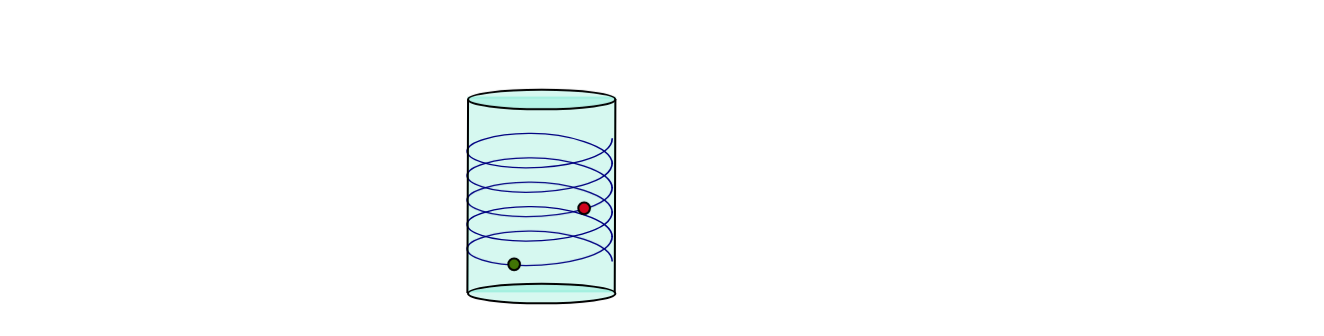
\includegraphics[scale=0.4]{pics/diagram-20250901.png} 
\end{figure}
\noindent
The invariant displacement for the cylinder can be written as $$ds^2 = r_0^2\dd\theta^2+\dd z^2$$
Note that the metric for this space is,
$$[g]\equiv \mqty(r_0^2 & 0 \\ 0 & 1)$$
This is a \textit{constant metric} which does not depend on the parameters $\theta$ or $z$. Then, all the Christoffel symbols will be zero since Christoffel symbols are essentially written in terms of the derivatives of the metric. The geodesic equations thus simplify to: 
$$\dv[2]{\theta}{\tau} = 0 \qquad \dv[2]{z}{\tau}=0$$
which have the solutions:
$$\theta = c_1\tau +c_2\qquad z = d_1\tau +d_2\implies z = d_1 \qty(\frac{\theta - c_2}{c_1})+d_2\implies z = m\theta + k$$
Suitably taking $k=0$, we see that the equation represents a helix with pitch $2\pi m$. Thus, the geodesics on the cylinder are helices and the shortest distance to move from one point to another on the cylinder is along a helix. \\[0.2cm]
NOTE: Similar to the case of the cylinder, for the flat spacetime, the metric is $\eta_{\mu\nu} = \mathrm{diag}(-1,+,+,+)$ which is constant too and hence, the geodesics for the Minkowski space will also satisfy the same equation as of the cylinder:
$$x^\mu = a^\mu + u^\mu\tau$$
where $u^\mu$ is the constant four-velocity and $a^\mu$ is the initial position (at $\tau=0$). This shows that geodesics in flat spacetime are straight lines.
